\documentclass[11pt]{scrreprt}


\usepackage{cmap}

\usepackage[utf8]{inputenc}
\usepackage[T1]{fontenc}
\usepackage[english, ngerman]{babel}

\usepackage{microtype}
\usepackage{csquotes}
\usepackage{enumitem}
\usepackage{amsmath}
\usepackage{amsthm}
\usepackage{amsfonts}
\usepackage{mathtools}

\usepackage{xpatch}
\makeatletter
\xpatchcmd{\proof}{\@addpunct{.}}{\@addpunct{:}}{}{}
\makeatother

\setlength{\parindent}{0cm}
\newcounter{thm}
\numberwithin{thm}{section}

\newtheorem{beispiel}[thm]{Beispiel}
\newtheorem{bemerkung}[thm]{Bemerkung}
\newtheorem{definition}[thm]{Definition}
\newtheorem{korollar}[thm]{Korollar}
\newtheorem{lemma}[thm]{Lemma}
\newtheorem{satz}[thm]{Satz}
\newtheorem{uebung}[thm]{Übung}

\newtheorem*{bemerkung*}{Bemerkung}
\newtheorem*{definition*}{Definition}
\newtheorem*{lemma*}{Lemma}
\newtheorem*{uebung*}{Übung}


\begin{document}


\chapter*{I. Unrestringierte Probleme}
\setcounter{chapter}{1}
\setcounter{section}{1}

\section*{Einführung}

\subsection*{Lösbarkeit}

\setcounter{section}{2}
\setcounter{thm}{2}

\begin{definition}[Lösbarkeit] ~\\
	Das Minimierungsproblem $P$ heißt \textbf{lösbar}, falls ein $\overline{x} \in M$ existiert mit
	$$ \inf_{x \in M} f(x) = f(\overline{x}) $$
\end{definition}

\setcounter{thm}{4}

\begin{satz}
	Das Minimierungsproblem $P$ ist genau dann lösbar, wenn es einen globalen Minimalpunkt besitzt.
\end{satz}

\begin{bemerkung*}
	Es können drei Fälle der Unlösbarkeit auftreten:

	\begin{itemize}
		\item $\inf_{x \in M} f(x) = + \infty$
		\item $\inf_{x \in M} f(x) = - \infty$
		\item Ein endliches Infimum wird nicht angenommen.
	\end{itemize}	
\end{bemerkung*}


\begin{satz}[Satz von Weierstraß] ~\\
	Die Menge $M \subseteq \mathbb{R}^n$ sei nichtleer und kompakt, und die Funktion $f \colon M \rightarrow \mathbb{R}$ sei stetig. Dann besitzt $f$ auf $M$ (mindestens) einen globalen Minimalpunkt und einen globalen Maximalpunkt.
\end{satz}

\setcounter{thm}{7}

\begin{definition}[Untere Niveaumenge]
	Für $X \subseteq \mathbb{R}^n, f \colon X \rightarrow \mathbb{R}$ und $\alpha \in \mathbb{R}$ heißt
	$$ \operatorname{lev}_{\leq}^{\alpha}(f, X) = \big\{ x \in X ~|~ f(x) \leq \alpha \big\} $$
	\textbf{untere Niveaumenge von $f$ auf $X$ zum Niveau $\alpha$}. Im Fall $X = \mathbb{R}^n$ schreiben wir auch kurz
	$$ f_{\leq}^{\alpha} \coloneqq \operatorname{lev}_{\leq}^{\alpha}(f, \mathbb{R}^n) = \big\{ x \in \mathbb{R}^n ~|~ f(x) \leq \alpha \big\} $$
\end{definition}

\setcounter{thm}{9}

\begin{uebung}
	Für eine abgeschlossene Menge $X \subseteq \mathbb{R}^n$ sei die Funktion $f \colon X \rightarrow \mathbb{R}$. Dann ist die Menge $\operatorname{lev}_{\leq}^{\alpha}(f, X)$ für alle $\alpha \in \mathbb{R}$ abgeschlossen.	
\end{uebung}

\begin{uebung}
	Für eine abgeschlossene Menge $X \subseteq \mathbb{R}^n$ und endliche Indexmengen $I$ und $J$ seien die Funktion $g_i \colon X \rightarrow \mathbb{R}, i \in I$, und $h_j \colon X \rightarrow \mathbb{R}, j \in J$, stetig. Dann ist die Menge 
		$$ M = \big\{ x \in X ~|~g_i(x) \leq 0, i \in I, ~ h_j(x) = 0, j \in J \big\} $$
		abgeschlossen.	
\end{uebung}

\begin{definition*}
	Die Menge der globalen Minimalpunkte lautet:
	$$ S = \big\{ \overline{x} \in M ~|~ \forall x \in M: f(x) \geq f(\overline{x}) \big\} $$
\end{definition*}

\begin{lemma}
	Für ein $\alpha \in \mathbb{R}$ sei $\operatorname{lev}_{\leq}^{\alpha}(f, M) \neq \emptyset$. Dann gilt 
	$$ S \subseteq \operatorname{lev}_{\leq}^{\alpha}(f, M). $$
\end{lemma}

\begin{satz}[Verschärfter Satz von Weierstraß]
	Für eine (nicht notwendigerweise beschränkte oder abgeschlossene) Menge $M \subseteq \mathbb{R}^n$ sei $f \colon M \rightarrow \mathbb{R}$ stetig, und mit einem $\alpha \in \mathbb{R}$ sei $\operatorname{lev}_{\leq}^{\alpha}(f, M)$ nichtleer und kompakt. Dann besitzt $f$ auf $M$ (mindestens) einen globalen Minimalpunkt.
\end{satz}

\setcounter{thm}{20}

\begin{definition}[Koerzivität]
	Gegeben seien eine abgeschlossene Menge $X \subseteq \mathbb{R}^n$ und eine Funktion $f \colon \mathbb{R}$ fall für alle Folgen $(x^k) \subseteq X$ mit $\lim_k \| x^k \| = +\infty$ auch
	$$ \lim_k f(x^k) = +\infty $$
	gilt, dann heißt $f$ \textbf{koerziv} auf $X$.
\end{definition}

\setcounter{thm}{23}

\begin{uebung}
		Gegeben sei die quadratische Funktion $q(x) = \frac{1}{2} x^T A x + b^T x$ mit einer symmetrischen $(n, n)$-Matrix $A$ (d.h. es gilt $A = A^T$) und $b \in \mathbb{R}^n$. Die Funktion $q$ ist genau dann koerziv auf $\mathbb{R}^n$, wenn $A$ positiv definit ist (d.h. wenn $d^T A d > 0$ für alle $d\in \mathbb{R}^n \setminus \{ 0 \}$ gilt).
\end{uebung}

\begin{beispiel}
	Auf kompakten Mengen $X$ ist jede Funktion $f$ trivialerweise koerziv.	
\end{beispiel}

\begin{lemma}
	Die Funktion $f \colon X \rightarrow \mathbb{R}$ sei stetig und koerziv auf der (nicht notwendigerweise beschränkten) abgeschlossenen Menge $X \subseteq \mathbb{R}^n$. Dann ist die Menge $\operatorname{lev}_{\leq}^{\alpha}(f, X)$ für jedes Niveau $\alpha \in \mathbb{R}$ kompakt.
\end{lemma}

\begin{korollar}
	Es sei $M$ nichtleer und abgeschlossen, aber nicht notwendigerweise beschränkt. Ferner sei die Funktion $f \colon M \rightarrow \mathbb{R}$ stetig und koerziv auf $M$. Dann besitzt $f$ auf $M$ (mindestens) einen globalen Minimalpunkt.
\end{korollar}

\subsection*{Rechenregeln und Umformungen}

\begin{uebung}[Skalare Vielfache und Summen]
	Gegeben seien $M \subseteq \mathbb{R}^n$ und $f,g \colon M \rightarrow \mathbb{R}$. Dann gilt
	\begin{enumerate}[label=\alph*\upshape)]
		\item $\forall \alpha \geq 0$, $\beta \in \mathbb{R} \colon \min_{x \in M} \left( \alpha f(x) + \beta \right) = \alpha \left( \min_{x \in M} f(x) \right) + \beta$
		\item $\forall \alpha <0$, $\beta \in \mathbb{R} \colon \min_{x \in M} \left( \alpha f(x) + \beta \right) = \alpha \left( \max_{x \in M} f(x) \right) + \beta$
		\item $\min_{x \in M} \left( f(x) + g(x) \right) \geq \min_{x \in M} f(x) + \min_{x \in M} g(x)$
	\end{enumerate}
\end{uebung}

\begin{uebung}[Separable Zielfunktion auf kartesischem Produkt]
	Es seien $X \subseteq \mathbb{R}^n$, $Y \subseteq \mathbb{R}^m$, $f \colon X \rightarrow \mathbb{R}$ und $g \colon Y \rightarrow \mathbb{R}$. Dann gilt
	$$ \min_{(x,y) \in X \times Y} \left( f(x) + g(y) \right) = \min_{x \in X} f(x) + \min_{y \in Y} g(y) $$	
\end{uebung}

\begin{uebung}[Vertauschung von Minima und Maxima]
	Es seien $X \subseteq \mathbb{R}^n$, $Y \subseteq \mathbb{R}^m$, $M = X \times Y$ und $f \colon M \rightarrow \mathbb{R}$ gegeben. Dann gilt:
	\begin{enumerate}[label=\alph*\upshape)]
		\item $\min_{(x,y) \in M} f(x, y) = \min_{x \in X} \min_{y \in Y} f(x,y) = \min_{y \in Y} \min_{x \in X} f(x, y)$
		\item $\max_{(x,y) \in M} f(x, y) = \max_{x \in X} \max_{y \in Y} f(x,y) = \max_{y \in Y} \max_{x \in X} f(x, y)$
		\item $\min_{x \in X} \max_{y \in Y} f(x, y) \geq \max_{y \in Y} \min_{x \in X} f(x, y)$
	\end{enumerate}
\end{uebung}

\begin{uebung}[Monotone Transformation]
	Zu $M \subseteq \mathbb{R}^n$ und einer Funktion $f \colon M \rightarrow Y$ mit $Y\subseteq \mathbb{R}$ sei $\psi \colon Y \rightarrow \mathbb{R}$ eine streng monoton wachsende Funktion. Dann gilt
	$$ \min_{x \in M} \psi \left( f(x) \right) = \psi \left( \min_{x \in M} f(x) \right), $$
	und die lokalen bzw. globalen Minimalpunkte stimmen überein.
\end{uebung}

\begin{uebung}[Epigraphumformulierung]
	Gegeben seien $M \subseteq \mathbb{R}^n$ und eine Funktion $f \colon M \rightarrow \mathbb{R}$. Dann sind die Probleme
	$$ P \colon \min_{x \in \mathbb{R}^n} f(x) \text{ s.t. } x \in M ~\text{ und } ~ P_{epi} \colon \min_{(x, \alpha) \in \mathbb{R}^n \times \mathbb{R}} \alpha \text{ s.t. } f(x) \leq \alpha, x \in M $$
	äquivalent, d.h. die Minimalwerte stimmen überein und Minimalpunkte entsprechen sich.
\end{uebung}

\begin{definition}[Parallelprojektion]
	Es sei $M \subseteq \mathbb{R}^n \times \mathbb{R}^m$. Dann heißt
	$$ \operatorname{pr}_x M = \big\{ x \in \mathbb{R}^n ~|~\exists y \in \mathbb{R}^m : (x, y) \in M \big\} $$
	\textbf{Parallelprojektion} von $M$ (den \enquote{$x$-Raum}) $\mathbb{R}^n$.
\end{definition}

\begin{uebung}[Projektionsumformulierung]
	Gegeben seien $M \subseteq \mathbb{R}^n \times \mathbb{R}^m$ und eine Funktion $f \colon \mathbb{R}^n \rightarrow \mathbb{R}$, die nicht von den Variablen aus $\mathbb{R}^m$ abhängt. Dann sind die Probleme 
	$$ P \colon \min_{(x, y) \in \mathbb{R}^n \times \mathbb{R}^m} f(x) ~\text{ s.t.} (x, y) \in M ~\text{ und } ~ P_{proj} \colon \min_{x \in \mathbb{R}^n} f(x) \text{ s.t. } x \in \operatorname{pr}_x M $$
	äquivalent, d.h. die Minimalwerte stimmen überein und Minimalpunkte entsprechen sich.
\end{uebung}

\setcounter{chapter}{2}
\setcounter{section}{1}

\newpage

\section*{Optimalitätsbedingungen}

\subsection*{Abstiegsrichtung}

\begin{definition}
	Es seien $f \colon \mathbb{R}^n \rightarrow \mathbb{r}$ und $\overline{x} \in \mathbb{R}^n$. Ein Vektor $d \in \mathbb{R}^n$ heißt \textbf{Abstiegsrichtung} für $f$ in $\overline{x}$, falls
	$$ \exists \hat{f} > 0 ~\forall t \in (0, \hat{t}) \colon f(\overline{x} + td) < f(\overline{x}). $$
\end{definition}

\begin{uebung}
	Für $f \colon \mathbb{R}^n \rightarrow \mathbb{R}$ sei $\overline{x}$ ein lokaler Minimalpunkt, dann kann keine Abstiegsrichtung für $f$ in $\overline{x}$ existieren.
\end{uebung}

\begin{definition}
	Gegeben seien $f \colon \mathbb{R}^n \rightarrow \mathbb{R}$, ein Punkt $\overline{x} \in \mathbb{R}^n$ und ein Richtungsvektor $d \in \mathbb{R}^n$. Die Funktion
	$$ \varphi_d \colon \mathbb{R}^1 \rightarrow
	 \mathbb{R}^1, ~ t \mapsto f(\overline{x} + td) $$
	 heißt \textbf{eindimensionale Einschränkung} von $f$ auf die durch $\overline{x}$ in Richtung $d$ verlaufende Gerade.
\end{definition}

\begin{bemerkung*}
		Es gilt $\varphi_d(0) = f(\overline{x})$ für jede Richtung $d \in \mathbb{R}^n$. Daher ist $d$ genau dann Abstiegsrichtung für $f$ in $\overline{x}$, wenn
		$$ \exists \hat{t} > 0 ~\forall t \in (0, \hat{t}) \colon \varphi_d(t) < \varphi_d(0) $$
\end{bemerkung*}

\subsection*{Optimalitätsbedingung erster Ordnung}

\begin{definition}
	Eine Funktion $f \colon \mathbb{R}^n \rightarrow \mathbb{R}$ heißt an $\overline{x} \in \mathbb{R}^n$ in eine Richtung $d \in \mathbb{R}^n$ \textbf{einseitig richtungsdifferenzierbar}, wenn der Grenzwert
	$$ f'(\overline{x}, d) \coloneqq \lim_{t \searrow 0} \frac{f(\overline{x} + td) - f(\overline{x})}{t} $$
	existiert. Der Wert $f'(\overline{x}, d)$ heißt dann \textbf{einseitige Richtungsableitung}. Die Funktion $f$ heißt an $\overline{x}$ einseitig richtungsdifferenzierbar, wenn $f$ an $\overline{x}$ in jede Richtung $d \in \mathbb{R}^n$ einseitig richtungsdifferenzierbar ist, und $f$ heißt \textbf{einseitig richtungsdifferenzierbar}, wenn $f$ an jedem $\overline{x} \in \mathbb{R}^n$ einseitig richtungsdifferenzierbar ist.
\end{definition}

\begin{lemma}
	Die Funktion $f \colon \mathbb{R}^n \rightarrow \mathbb{R}$ sei an $\overline{x} \in \mathbb{R}^n$ in Richtung $d \in \mathbb{R}^n$ einseitig richtungsdiffrenzierbar mit $f'(\overline{x}, d) < 0$. Dann ist $d$ Abstiegsrichtung für $f$ in $\overline{x}$.	
\end{lemma}

\begin{lemma}
	Die Funktion $f \colon \mathbb{R}^n \rightarrow \mathbb{R}$ sei an einem lokalen Minimalpunkt $\overline{x} \in \mathbb{R}^n$ einseitig richtungsdifferenzierbar. Dann gilt $f'(\overline{x}, d) \geq 0$ für jede Richtung $d \in \mathbb{R}^n$l
\end{lemma}

\begin{definition}[Abstiegsrichtung erster Ordnung]
	Für eine am Punkt $\overline{x} \in \mathbb{R}^n$ in Richtung $d \in \mathbb{R}^n$ einseitig richtungsdifferenzierbare Funktion $f \colon \mathbb{R}^n \rightarrow \mathbb{R}$ heißt $d$ \textbf{Abstiegsrichtung erster Ordnung}, falls $f'(\overline{x}, d) < 0$ gilt.	
\end{definition}

\begin{definition}[Stationärer Punkt - unrestringierter Fall]
	Die Funktion $f \colon \mathbb{R}^n \rightarrow \mathbb{R}$ sei an $\overline{x} \in \mathbb{R}^n$ einseitig richtungsdifferenzierbar. Dann heißt $\overline{x}$ \textbf{stationärer Punkt} von $f$, falls $f'(\overline{x}, d) \geq 0$ für jede Richtung $d \in \mathbb{R}^n$ gilt.
\end{definition}

\begin{satz}[Kettenregel]
	Es seien $g \colon \mathbb{R}^n \rightarrow \mathbb{R}^m$ differenzierbar an $\overline{x} \in \mathbb{R}^n$ und $f \colon \mathbb{R}^m \rightarrow \mathbb{R}^k$ differenzierbar an $g(\overline{x}) \in \mathbb{R}^m$. Dann ist $f \circ g \colon \mathbb{R}^n \rightarrow \mathbb{R}^k$ differenzierbar an $\overline{x}$ mit
	$$ D( f \circ g )(\overline{x}) = D f( g(\overline{x}) ) \cdot D g(\overline{x}). $$
\end{satz}

\begin{lemma}
	Die Funktion $f \colon \mathbb{R}^n \rightarrow \mathbb{R}$ sei am Punkt $\overline{x} \in \mathbb{R}^n$ differenzierbar, und für die Richtung $d \in \mathbb{R}^n$ gelte $\langle \nabla f(\overline{x}), d \rangle < 0$. Dann ist $d$ Abstiegsrichtung für $f$ in $\overline{x}$.
\end{lemma}

\begin{bemerkung}
	Ein Vektor $d$ ist genau dann eine Abstiegsrichtung erster Ordnung für $f$ in $\overline{x}$, wenn $d$ einen stumpfen Winkel mit dem Gradienten $\nabla f(\overline{x})$ bildet. Wobei das Skalarprodukt genau dann negativ, wenn sie einen stumpfen Winkel miteinander bilden, und analog ist das Skalarprodukt genau für einen spitzen Winkel bildende Vektoren positiv.	
\end{bemerkung}

\begin{uebung}
	Gegeben seien $\overline{x} \in \mathbb{R}^n$, eine endliche Indexmenge $K$ und an $\overline{x}$ differenzierbare Funktionen $f_k \colon \mathbb{R}^n\rightarrow \mathbb{R}$, $k \in K$. Die Funktion $f(x) \coloneqq \max_{k \in K} f_k(x)$ ist an $\overline{x}$ einseitig richtungsdifferenzierbar und dass mit $K_*(\overline{x}) = \{ k \in K ~|~f_k(\overline{x}) = f(\overline{x}) \}$
	$$ f'(\overline{x}, d) = \max_{k \in K_x(\overline{x})} \langle \nabla f_k(\overline{x}), d \rangle $$
	für jede Richtung $d \in \mathbb{R}^n$ gilt.
\end{uebung}

\begin{satz}[Notwendige Optimalitätsbedingung erster Ordnung – Fermat'sche Regel]
	Die Funktion $f \colon \mathbb{R}^n \rightarrow \mathbb{R}$ sei differenzierbar an einem lokalen Minimalpunkt $\overline{x} \in \mathbb{R}$. Dann gilt $\nabla f(\overline{x}) = 0$.
\end{satz}

\begin{definition}[Kritischer Punkt]
	Die Funktion $f \colon \mathbb{R}^n \rightarrow \mathbb{R}$ sei an $\overline{x} \in \mathbb{R}^n$ differenzierbar. Dann heißt $\overline{x}$ kritischer Punkt von $f$, wenn $\nabla f(\overline{x}) = 0$ gilt.
\end{definition}

\begin{uebung}
	Die Funktion $f \colon \mathbb{R}^n \rightarrow \mathbb{R}$ sei differenzierbar an einem Punkt $\overline{x} \in \mathbb{R}^n$. Der Punkt $\overline{x}$ ist genau dann stationärer Punkt von $f$, wenn er kritischer Punkt von $f$ ist.	
\end{uebung}

\setcounter{thm}{16}

\begin{definition}[Sattelpunkt]
	Die Funktion $f \colon \mathbb{R}^n \rightarrow \mathbb{R}$ sei an $\overline{x} \in \mathbb{R}^n$ differenzierbar. Dann heißt $\overline{x}$ \textbf{Sattelpunkt} von $f$, falls $\overline{x}$ zwar kritischer Punkt von $f$, aber weder lokaler Minimal- noch lokaler Maximalpunkt ist.
\end{definition}

\subsection*{Geometrische Eigenschaften von Gradienten}

\begin{center}
	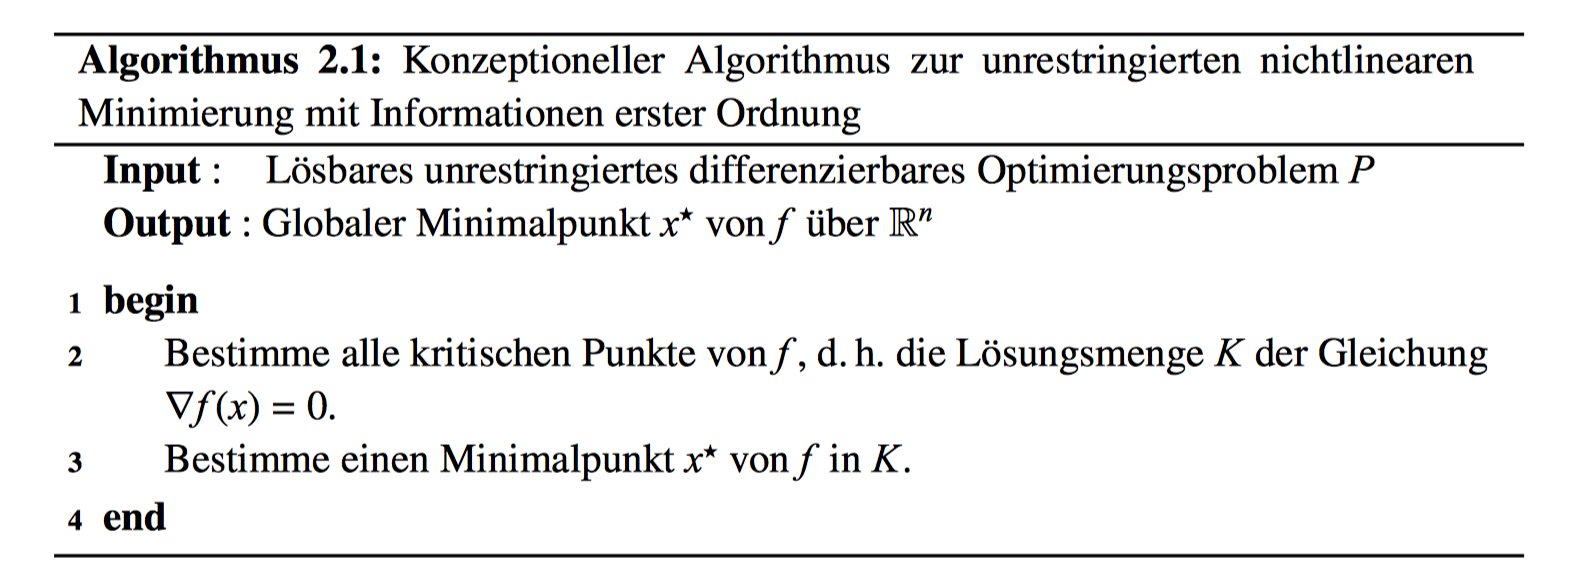
\includegraphics[scale=0.5]{a21}
\end{center}

\begin{center}
	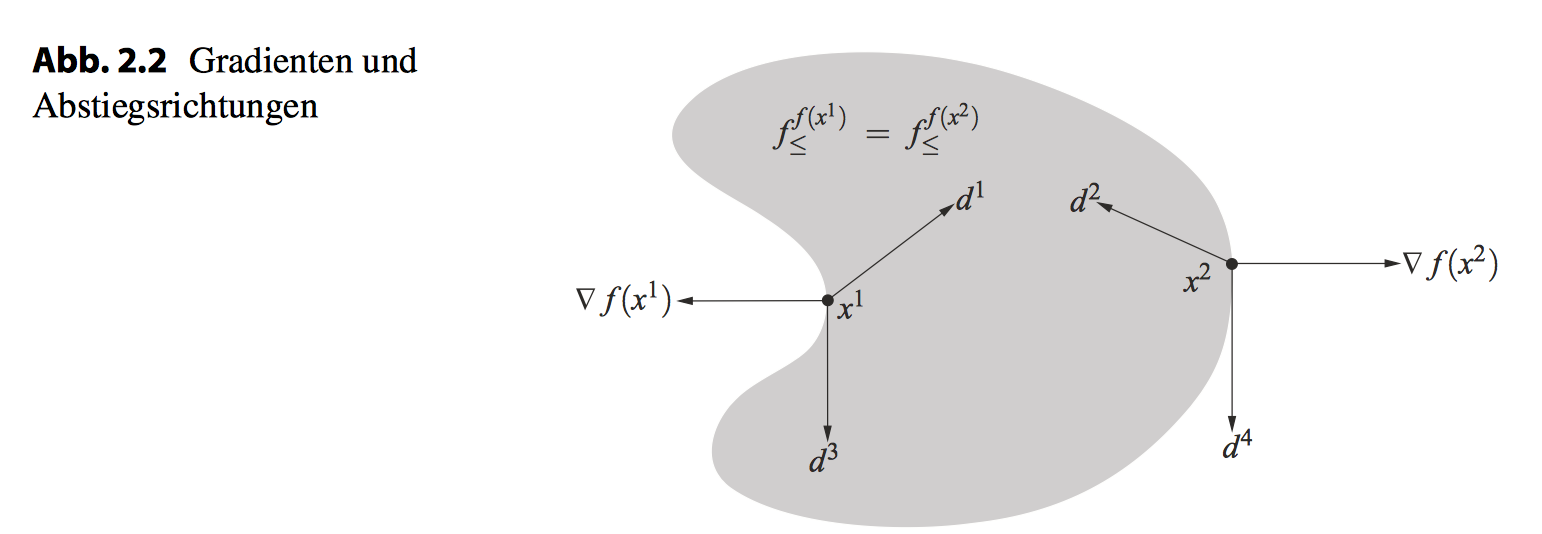
\includegraphics[scale=0.4]{ab22}
\end{center}

\setcounter{thm}{18}

\begin{bemerkung*}
	Man kann zeigen, dass jeder Vektor $d \in \mathbb{R}^n$ mit $\langle \nabla f(\overline{x}), d \rangle > 0$ eine Anstiegsrichtung erster Ordnung ist. Da für einen nichtkritischen Punkt $\overline{x}$ die Gradientenrichtung $d =\nabla f(\overline{x})$ die strikte Ungleichung
	$$ \langle \nabla f(\overline{x}), \nabla f(\overline{x}) \rangle = \{ \nabla f(\overline{x}) \|_2^2 > 0 $$
	erfüllt, ist $d = \nabla f(\overline{x})$ also eine Anstiegsrichtung erster Ordnung für $f$ in $\overline{x}$, und man kann zeigen, dass $\nabla f(\overline{x})$ senkrecht auf dem Rand von $f_{\leq}^{f(\overline{x})}$ steht.
\end{bemerkung*}

\subsection*{Optimalitätsbedingungen zweiter Ordnung}

\begin{bemerkung*}
	Für normierte Richtungen $d$ liefert die Cauchy-Schwarz-Ungleichung 
	$$ - \| \nabla f(\overline{x}) \|_2 = -  \| \nabla f(\overline{x}) \|_2 \cdot \| d \|_2 \leq \langle \nabla f(\overline{x}), d \rangle \leq \| \nabla f(\overline{x}) \|_2 \cdot \| d \|_2 = \| \nabla f(x) \|_2 $$
	und die Unter- und Oberschranken werden genau für linear abhängige $d$ und $\nabla f(\overline{x})$ angenommen. Wegen $\nabla f(\overline{x})$ wird die kleinst- und größtmögliche Steigung daher folgend realisiert
	$$ d_{min} = - \frac{\nabla f(\overline{x})}{\| \nabla f(\overline{x}) \|_2} ~\text{ und }~ d_{max} = \frac{\nabla f(\overline{x})}{\| \nabla f(\overline{x}) \|_2}  $$	
	In der Praxis arbeitet man aber nicht mit der negativen Gradientenrichtung, denn gerade in der Nähe der gesuchten kritischen Punkte - nahe bei null - ist die Division $\frac{\nabla f(\overline{x})}{\| \nabla f(\overline{x}) \|_2}$ numerisch instabil.
\end{bemerkung*}

\begin{satz}[Entwicklungen 1. und 2. Ordnung per univariatem Satz von Taylor] ~\
	\begin{enumerate}[label=\alph*\upshape)]
		\item Es sei $\varphi \colon \mathbb{R} \rightarrow \mathbb{R}$ differenzierbar an $\overline{t}$. Dann gilt für alle $t \in \mathbb{R}$
			$$ \varphi(t) = \varphi(\overline{t}) + \varphi'(\overline{t})(t-\overline{t}) + o(|t - \overline{t}|), $$
			wobei $o(|t-\overline{t}|)$ einen Ausdruck der Form $\omega(t) \cdot |t-\overline{t}|$ mit $\lim_{t \rightarrow \overline{t}} \omega(t) = \omega(\overline{t}) = 0$ bezeichnet.
		\item Es sei $\varphi \colon \mathbb{R} \rightarrow \mathbb{R}$ zweimal differenzierbar an $\overline{t}$. Dann gilt für alle $t \in \mathbb{R}$
			$$\varphi(t) = \varphi(\overline{t}) + \varphi'(\overline{t})(t - \overline{t}) + \frac{1}{2} \varphi''(\overline{t})(t-\overline{t})^2 + o(|t-\overline{t}|^2), $$
			wobei $o(|t-\overline{t}|^2)$ einen Ausdruck der Form $\omega(t) \cdot |t-\overline{t}|^2$ mit $\lim_{t \rightarrow \overline{t}} \omega(t) = \omega(\overline{t}) = 0$ bezeichnet.
	\end{enumerate}
\end{satz}

\begin{lemma}
	Für $f \colon \mathbb{R}^n \rightarrow \mathbb{R}$, einen Punkt $\overline{x} \in \mathbb{R}^n$ und eine Richtung $d \in \mathbb{R}^n$ seien $\varphi'_d(0) = 0$ und $\varphi_d''(0) < 0$. Dann ist $d$ Abstiegsrichtung für $f$ in $\overline{x}$.
\end{lemma}

\begin{lemma}
	Für $f \colon \mathbb{R}^n \rightarrow \mathbb{R}$ sei $\overline{x}$ ein lokaler Minmalpunkt. Dann gilt $\nabla f(\overline{x}) = 0$, und jede Richtung $d \in \mathbb{R}^n$ erfüllt $\varphi_d''(0) \geq 0$.
\end{lemma}

\begin{bemerkung*}
		Es gilt für eine Richtung $d$ gilt, dass $\varphi_d''(0) = d^T D^2 f(\overline{x}) d$
\end{bemerkung*}

\begin{lemma}
	Für $f \colon \mathbb{R}^n \rightarrow \mathbb{R}$, einen Punkt $\overline{x} \in \mathbb{R}^n$ und eine Richtung $d \in \mathbb{R}^n$ seien $\langle \nabla f(\overline{x}), d \rangle = 0$ und $d^T D^2 f(\overline{x}) d < 0$. Dann ist $d$ Abstiegsrichtung für $f$ in $\overline{x}$.
\end{lemma}

\begin{definition}[Abstiegsrichtung zweiter Ordnung]
	Zu $f \colon \mathbb{R}^n \rightarrow \mathbb{R}$ und $\overline{x} \in \mathbb{R}^n$ heißt jeder Richtungsvektor $d \in \mathbb{R}^n$ mit $\langle \nabla f(\overline{x}), d \rangle = 0$ und $d^T D^2 f(\overline{x}) d < 0$ \textbf{Abstiegsrichtung zweiter Ordnung} für $f$ in $\overline{x}$.
\end{definition}

\setcounter{thm}{26}

\begin{satz}[Notwendige Optimalitätsbedingung zweiter Ordnung] ~\
	Die Funktion $f \colon \mathbb{R}^n \rightarrow \mathbb{R}$ sei zweimal differenzierbar an einem lokalen Minimalpunkt $\overline{x} \in \mathbb{R}^n$. Dann gilt $\nabla f(\overline{x}) = 0$ und $D^2 f(\overline{x}) \succeq 0$.	
\end{satz}

\begin{center}
	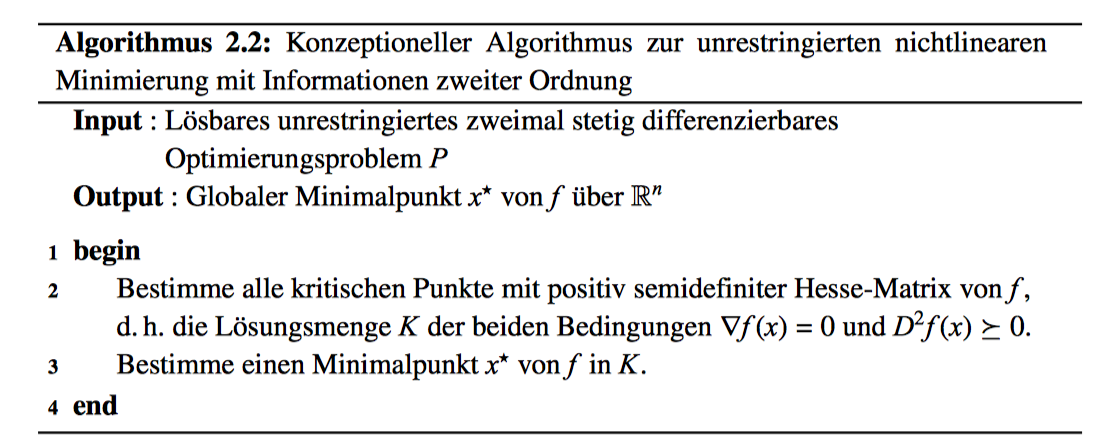
\includegraphics[scale=0.5]{a22}
\end{center}

\setcounter{thm}{29}

\begin{satz}[Entwicklungen 1. und 2. Ordnung per univariatem Satz von Taylor] ~\
	\begin{enumerate}[label=\alph*\upshape)]
		\item Es sei $f \colon \mathbb{R}^n \rightarrow \mathbb{R}$ differenzierbar an $\overline{x}$. Dann gilt für alle $x \in \mathbb{R}^n$
			$$ f(x) = f(\overline{x}) + \langle \nabla f(\overline{x}), x -\overline{x} \rangle + o(\|x - \overline{x}\|), $$
			wobei $o(\|x-\overline{x}\|)$ einen Ausdruck der Form $\omega(x) \cdot \|x-\overline{x}|$ mit $\lim_{x \rightarrow \overline{x}} \omega(x) = \omega(\overline{x}) = 0$ bezeichnet.
		\item Es sei $f \colon \mathbb{R}^n \rightarrow \mathbb{R}$ zweimal differenzierbar an $\overline{x}$. Dann gilt für alle $x \in \mathbb{R}^n$
			$$ f(x) = f(\overline{x}) + \langle f(\overline{x}), x - \overline{x} \rangle + \frac{1}{2} (x-\overline{x})^T D^2 f(\overline{x}) (x-\overline{x}) + o(\|x-\overline{x}\|^2), $$
			wobei $o(\|x-\overline{x}\|^2)$ einen Ausdruck der Form $\omega(x) \cdot \|x-\overline{x}\|^2$ mit $\lim_{x \rightarrow \overline{x}} \omega(x) = \omega(\overline{x}) = 0$ bezeichnet.
	\end{enumerate}
\end{satz}

\begin{definition*} ~\
	\begin{itemize}
		\item $B_{\leq}(\overline{x}, r) = \big\{ x \in \mathbb{R}^n ~|~ \| x - \overline{x} \| \leq r \big\}$
		\item $B_{=}(\overline{x}, r) = \big\{ x \in \mathbb{R}^n ~|~ \| x - \overline{x} \| = r \big\}$
	\end{itemize}	
\end{definition*}

\begin{satz}[Hinreichende Optimalitätsbedingung zweiter Ordnung]
	Die Funktion $f \colon \mathbb{R}^n \rightarrow \mathbb{R}$ sei an $\overline{x} \in \mathbb{R}^n$ zweimal differenzierbar, und es gelte $\nabla f(\overline{x}) = 0$ und $D^2 f(\overline{x}) \succ 0$. Dann ist $\overline{x}$ ein strikter lokaler Minimalpunkt von $f$.
\end{satz}

\setcounter{thm}{34}

\begin{definition}[Nichtdegenerierte kritische und Minimalpunkt] ~\
	Die Funktion $f \colon \mathbb{R}^n \rightarrow \mathbb{R}$ sei an $\overline{x}$ zweimal differenzierbar mit $\nabla f(\overline{x}) = 0$. Dann heißt $\overline{x}$
	\begin{enumerate}[label=\alph*\upshape)]
		\item \textbf{nichtdegenerierter kritischer Punkt}, falls $D^2 f(\overline{x})$ nichtsingulär ist,
		\item \textbf{nichtdegenerierter lokaler Minimalpunkt}, falls $\overline{x}$ lokaler Minimalpunkt und nichtdegenerierter kritischer Punkt ist.
	\end{enumerate}	
\end{definition}

\begin{lemma}
	Der Punkt $\overline{x}$ ist genau dann nichtdegenerierter lokaler Minimalpunkt von $f$, wenn $\nabla f(\overline{x}) = 0$ und $D^2 f(\overline{x}) \succ 0$ gilt.
\end{lemma}

\begin{definition*}
	$\mathcal{F} = \big\{ f \in C^2(\mathbb{R}^n, \mathbb{R}) ~|$ alle kritischen Punkte von $f$ sind nichtdegeneriert $\big\}$	
\end{definition*}

\begin{satz}
	$\mathcal{F}$ ist $C_s^2$-offen und -dicht in $C^2(\mathbb{R}^n, \mathbb{R})$.
\end{satz}

\begin{uebung}
	In einem nichtdegeneriertem Sattelpunkt existiert sowohl eine Ab- als auch eine Anstiegsrichtung zweiter Ordnung.
\end{uebung}

\subsection*{Konvexe Optimierungsprobleme}

\begin{definition}[Konvexe Mengen und Funktionen] ~\
	\begin{enumerate}[label=\alph*\upshape)]
		\item Eine Menge $X \subseteq \mathbb{R}^n$ heißt \textbf{konvex}, falls
			$$ \forall x,y \in X, \lambda \in (0, 1): \quad (1-\lambda) x + \lambda y \in X $$
			gilt (d.h. die Verbindungsstrecke von je zwei beliebigen Punkten in $X$ gehört komplett zu $X$).
		\item Für eine konvexe Menge $X \subseteq \mathbb{R}^n$ heißt eine Funktion $f \colon X \rightarrow \mathbb{R}$ \textbf{konvex} (auf $X$), falls
			$$ \forall x, y \in X, \lambda \in (0, 1): \quad f((1-\lambda) x + \lambda y) \leq (1-\lambda) f(x) + \lambda f(y) $$
			gilt (d.h. der Funktionsgraph von $f$ verläuft unter jeder seiner Sekanten).
	\end{enumerate}
\end{definition}

\begin{bemerkung*}
	Während die Konvexität einer Funktion geometrisch dadurch definiert ist, dass ihr Graph unter jeder ihrer Sekanten verläuft, lässt sich Konvexität einer stetig differenzierbaren Funktion $f$ dadurch charakterisieren, dass ihr Graph über den Graphen jeder ihrer Linearisierungen verläuft.	
\end{bemerkung*}

\begin{center}
	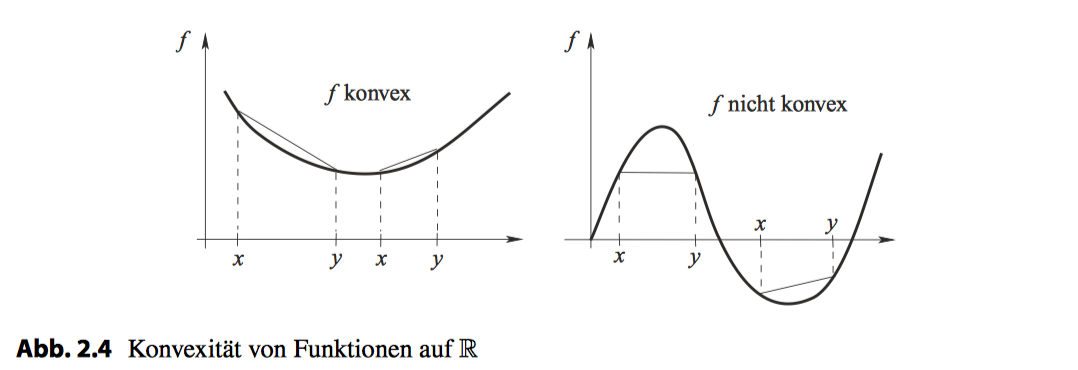
\includegraphics[scale=0.5]{ab24}
\end{center}

\begin{satz}[$C^1$-Charakterisierung von Konvexität]
	Auf einer konvexen Menge $X \subseteq \mathbb{R}^n$ ist eine Funktion $f \in C^1(X, \mathbb{R})$ genau dann konvex, wenn folgendes gilt:
	$$ \forall x,y \in X: \quad f(y) \geq f(x) + \langle \nabla f(x) , y - x \rangle $$	
\end{satz}

\begin{korollar}
	Die Funktion $f \in C^1(\mathbb{R}^n, \mathbb{R})$ sei konvex. Dann sind die kritischen Punkte von $f$ genau die globalen Minimalpunkte von $f$.
\end{korollar}

\begin{satz}[$C^2$-Charakterisierung von Konvexität]
	Eine Funktion $f \in C^2(\mathbb{R}^n, \mathbb{R})$ ist genau dann konvex, wenn folgendes gilt:
	$$ \forall x \in \mathbb{R}^n: \quad D^2 f(x) \succeq 0 $$	
\end{satz}

\begin{uebung}
	Gegeben sei die quadratische Funktion $q(x) = \frac{1}{2} x^T A x + b^T x$ mit $A = A^T \succ 0$ und $b \in \mathbb{R}^n$. Die Funktion $q$ ist eine auf $\mathbb{R}^n$ (gleichmäßige) konvexe Funktion und ihr eindeutiger Minimalpunkt 
	$$ x^* = - A^{-1} b $$
	mit Minimalwert $q(x^*) = - \frac{1}{2}b^T A^{-1} b$.
\end{uebung}

\section*{Numerische Verfahren}

\setcounter{section}{2}
\setcounter{thm}{0}

\subsection{Abstiegsverfahren}
Zunächst betrachten wir Verfahren, die in jedem Iterationsschritt einen Abstieg im Zielfunktionswert erzeugen, für die also

$$ \forall k \in \mathbb{N}_0: \quad f(x^{k+1}) < f(x^k) $$

gilt. Solche Verfahren können nur \enquote{unter sehr unglücklichen Umständen} gegen lokale Maximalpunkte konvergieren und aus geometrischen Überlegungen heraus ist die Konvergenz gegen Sattelpunkte unwahrscheinlich. ~\bigskip

Neben der Stetigkeit der Zielfunktion $f$ werden wir im gesamten Abschn. 2.2 fordern, dass die untere Niveaumenge $f_{\leq}^{f(x^0)}$ zum Startpunkt $x^0 \in \mathbb{R}^n$ beschränkt ist.

\begin{uebung*}
	Als erste algorithmische Idee könnte man versuchen, die Gleichung $\nabla f(x) = 0$ mit dem aus der Numerik bekannten Newton-Verfahren

	$$ x^{k+1} = x^k - \left( D^2 f(x^k) \right)^{-1} \nabla f(x^k), \quad k = 0, 1, 2, \dotsc $$
	
	Vorteil wäre eine hohe Konvergenzgeschwindigkeit, falls $x^0$ nahe genug an einer Lösung liegt. Nachteilig ist, dass $x^0$ nicht in der Nähe einer Lösung zu liegen braucht, dass die Hesse-Matrix $D^2 f ( x^k )$ nicht notwendig invertierbar sein muss und dass das Newton-Verfahren auch gegen lokale Maximalpunkte und Sattelpunkte konvergieren kann.
\end{uebung*}

\begin{center}
	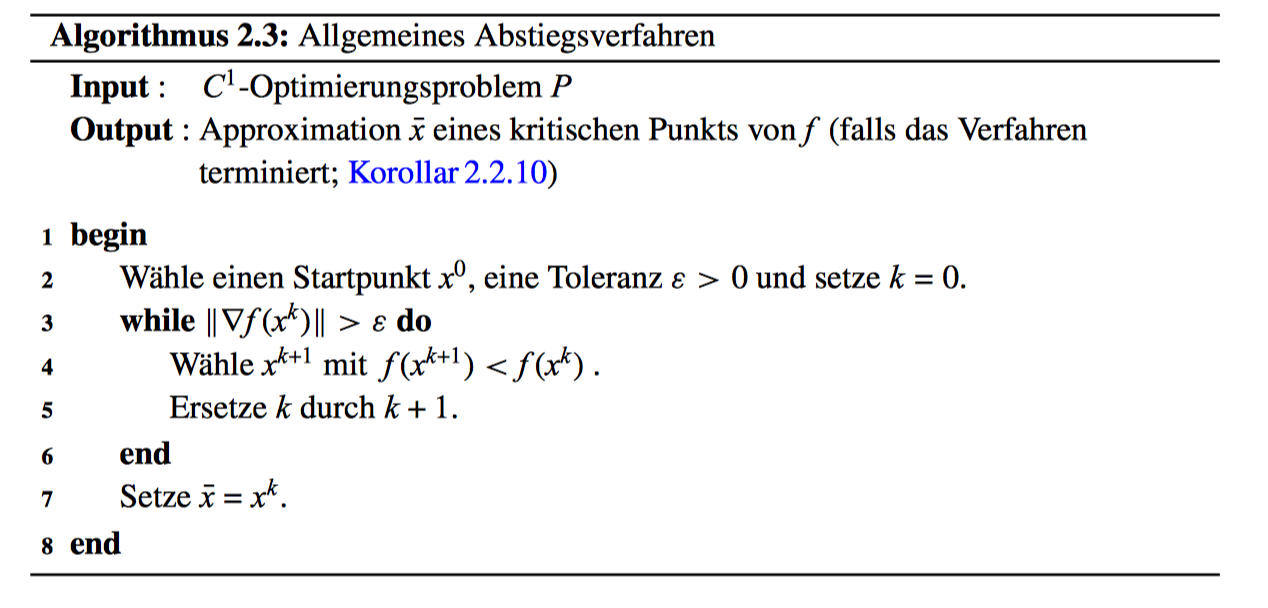
\includegraphics[scale=0.4]{a23}
\end{center}

\setcounter{thm}{2}

\begin{lemma}
	Für beschränktes $f_{\leq}^{f(x^0)}$ bricht die von Algorithmus 2.3 mit $\epsilon = 0$ erzeugte Folge $(x^k)$ entweder nach endlich vielen Schritten mit einem kritischen Punkt ab, oder sie besitzt mindestens einen Häufungspunkt in $f_{\leq}^{f(x^0)}$, und die Folge der Funktionswerte $\left( f(x^k) \right)$ ist konvergent.
\end{lemma}

\setcounter{thm}{4}

\begin{definition}[Effiziente Schrittweiten]
	Es sei $(d^k)$ eine Folge von Abstiegsrichtungen erster Ordnung, und $(t^k)$ erfülle
	$$ \exists c > 0 ~\forall k \in \mathbb{N}: \quad f(x^k+ t^k d^k) - f(x^k) \leq -c \left( \frac{\langle \nabla f(x^k) , d^k \rangle}{\| d^k \|_2} \right)^2 $$
	Dann heißt $(t^k)$ \textbf{effiziente Schrittweitenfolge} für $(d^k)$.
\end{definition}

\begin{satz}
	Die Menge $f_{\leq}^{f(x^0)}$ sei beschränkt, $(d^k)$ sei eine Folge von Abstiegsrichtungen erster Ordnung, und $(t^k)$ sei eine effiziente Schrittweitenfolge. Dann gilt (2.6):
	$$ \lim_{k} \frac{\langle \nabla f(x^k), d^k \rangle}{\| d^k \|_2}	= 0. $$
\end{satz}

\begin{definition}[Gradientenbezogene Suchrichtungen]
	Die Folge von Suchrichtungen $(d^k)$ heißt \textbf{gradientenbezogen}, falls folgendes gilt:
	$$ \exists c > 0 ~\forall k \in \mathbb{N}: \quad \frac{\langle \nabla f(x^k), d^k \rangle}{\| d^k \|_2} \leq - c \cdot \| \nabla f(x^k)\|_2 $$
\end{definition}

\begin{uebung}
	Die Suchrichtungen $d^k = - \nabla f(x^k)$, $k \in \mathbb{N}$ sind gradientenbezogen.
\end{uebung}

\begin{satz}
	Die Menge $f_{\leq}^{f(x^0)}$ sei beschränkt, und in Zeile 4 von Algorithmus 2.3 sei $x^{k+1} = x^k + t^k d^k$ mit einer gradientenbezogenen Suchrichtungsfolge $(d^k)$ und einer effizienten Schrittweitenfolge $(t^k)$ gewählt. Für $\epsilon = 0$ stoppt dann das Verfahren entweder nach endlich vielen Schritten mit einem kritischen Punkt, oder die Folge $(x^k )$ besitzt einen Häufungspunkt, und für jeden solchen Punkt $x^*$ gilt $\nabla f(x^*) = 0$.	
\end{satz}

\begin{korollar}
	Die Menge $f_{\leq}^{f(x^0)}$ sei beschränkt, und in Zeile 4 von Algorithmus 2.3 sei $x^{k+1} = x^k + t^k d^k$ mit einer gradientenbezogenen Suchrichtungsfolge $(d^k)$ und einer effizienten Schrittweitenfolge $(t^k)$ gewählt. Dann terminiert das Verfahren für jedes $\epsilon > 0$ nach endlich vielen Schritten.
\end{korollar}

\subsection*{Schrittweitensteuerung}

\begin{definition*}
	Eine Funktion $F \colon D \rightarrow \mathbb{R}^m$ heißt \textbf{Lipschitz-stetig} auf $D \subseteq \mathbb{R}^n$, falls
	$$ \exists L > 0 ~\forall x, y \in D: \quad \| F(x) - F(y) \|_2 \leq L \cdot \| x - y \|_2 $$
	$C^1$-Funktionen sind auf kompakten Mengen immer Lipschitz-stetig sind, damit ist $\nabla f$ bei beschränkter Menge $f_{\leq}^{f(x^0)}$ zum Beispiel für jede $C^2$-Funktion $f$ Lipschitz-stetig auf $f_{\leq}^{f(x^0)}$.
\end{definition*}

\setcounter{thm}{11}

\begin{bemerkung}
	Bei beschränktem (und daher kompaktem) $f_{\leq}^{f(x^0)}$ ist die Menge $\operatorname{conv}(f_{\leq}^{f(x^0)})$ ebenfalls kompakt, so dass die Forderung der Lipschitz-Stetigkeit von $\nabla f$ auch auf $\operatorname{conv}(f_{\leq}^{f(x^0)})$ eine schwache Voraussetzung ist.	
\end{bemerkung}

\begin{lemma}
	Auf einer konvexen Menge $D \subseteq \mathbb{R}^n$ sei $f$ differenzierbar mit Lipschitz-stetigem Gradienten $\nabla f$ und zugehöriger Lipschitz-Konstante $L > 0$. Dann gilt
	$$ \nabla \overline{x}, x \in D: \quad \left| f(x) - f(\overline{x})- \langle \nabla f(\overline{x}), x - \overline{x} \rangle \right| \leq \frac{L}{2} \| x - \overline{x} \|_2^2 $$
\end{lemma}

\subsubsection*{Exakte Schrittweiten}

Zu $x \in f_{\leq}^{f(x^0)}$ sei eine Abstiegsrichtung erster Ordnung $d$ für $f$ in $x$ gegeben. Wegen $\varphi_d'(0) = \langle \nabla f(x), d \rangle < 0$ gilt $\varphi_d(t) < \varphi_d(0)$ für kleine positive $t$. Für beschränktes $f_{\leq}^{f(x^0)}$ besitzt $\varphi_d$ nach dem Satz von Weierstraß sogar globale Minimalpunkte $t_e> 0$, die exakte Schrittweiten genannt werden. Per Definition der eindimensionalen Einschränkung $\varphi_d$ erfüllen sie
$$ f(x + t_e d) = \min_{t > 0} f(x + td) $$

Eine exakte Schrittweite zu berechnen, um den größtmöglichen Abstieg von $x$ aus entlang d zu erzielen, ist im Allgemeinen sehr aufwendig, so dass wir dieses Konzept meist nur für theoretische Zwecke benutzen werden und später stattdessen zu inexakten Schrittweiten übergehen werden. 

\begin{uebung}
	Gegeben sei die quadratische Funktion $q(x) = \frac{1}{2} x^T A x + b^T x$ mit $A = A^T \succ 0$ und $b \in \mathbb{R}^n$, die nach Übung 1.2.24 koerziv und nach Übung 2.1.43 konvex ist. Für 
	jedes $x \in \\mathbb{R}^n$ und jede Abstiegsrichtung erster Ordnung $d$ 
	für $q$ in $x$ die exakte Schrittweite eindeutig bestimmt zu
	$$ t_e = - \frac{\langle Ax + b, d \rangle}{d^T A d} $$
\end{uebung}

\begin{satz}
	Die Menge $f_{\leq}^{f(x^0)}$ sei beschränkt, die Funktion $\nabla f$ sei Lipschitz-stetig auf $\operatorname{conv}(f_{\leq}^{f(x^0)})$, und $(d^k)$ sei eine Folge von Abstiegsrichtung erster Ordnung. Dann ist jede Folge von exakten Schrittweiten $(t_e^k)$ effizient.
\end{satz}

\subsubsection*{Konstante Schrittweiten}

Falls die Funktion f keine besondere Struktur aufweist, lohnt sich der Aufwand nicht, in jedem Iterationsschritt eine exakte Schrittweite $t_e^k$ zu berechnen. Daher bnutzt man dann lieber inexakte Schrittweiten, die ebenfalls effizient, aber erheblich leichter zu berechnen sind. ~\bigskip

Eine zunächst naheliegend erscheinende Möglichkeit dafür besteht darin 
 $$ t_c^k = - \frac{\langle \nabla f(x^k), d^k \rangle}{L \cdot \|d^k \|_2^2} $$
Auch diese Schrittweitre ist effizient, genauso wie die exakte. Im speziellen Fall $d^k = -\nabla f (x^k)$ gilt sogar

	$$ t_c^k = \frac{1}{L} $$
	

\subsubsection*{Armijo-Schrittweiten}
	
Eine in modernen Implementierungen von Optimierungsverfahren sehr beliebte inexakte Schrittweitensteuerung geht auf eine Idee von Armijo zurück: Zu $x \in f_{\leq}^{f(x^0)}$ seien $d$ eine Abstiegsrichtung erster Ordnung und $\sigma \in (0,1)$. Dann existiert ein $t > 0$, so dass für alle $t \in (0, \hat{t})$ die Werte $\varphi_d(t)$ unter der \enquote{nach oben gedrehten Tangente} $\varphi_d(0) + t \sigma \varphi_d'(0)$ liegen, so dass also gilt:	
	$$ f(x + td) \leq f(x) + t \sigma \langle \nabla f(x), d \rangle $$
	
	Offensichtlich erfüllt jedes solche $t$££ die Bedingung (2.3):
	$$ \exists c_1 > 0 ~\forall k\in \mathbb{N}: \quad f(x^k + t^k d^k) - f(x^k) \leq c_1 \cdot t^k \langle \nabla f(x^k), d^k \rangle $$
	 mit $c_1 = \sigma$.
	
\begin{center}
	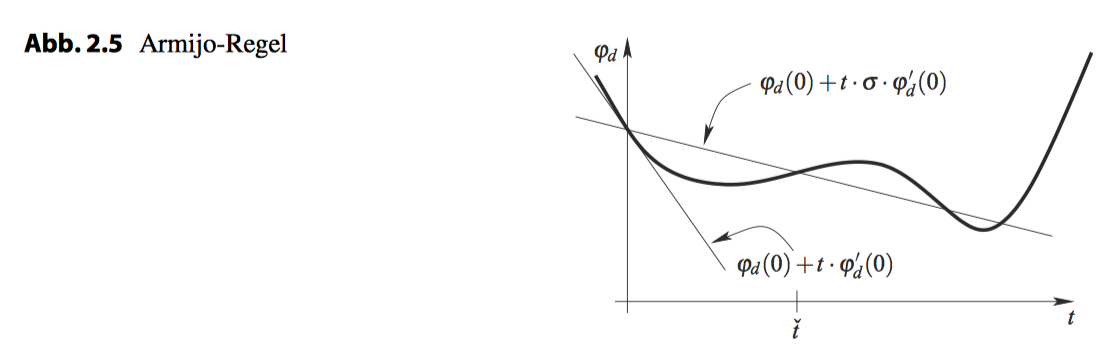
\includegraphics[scale=0.5]{ab25}
\end{center}	

\begin{center}
	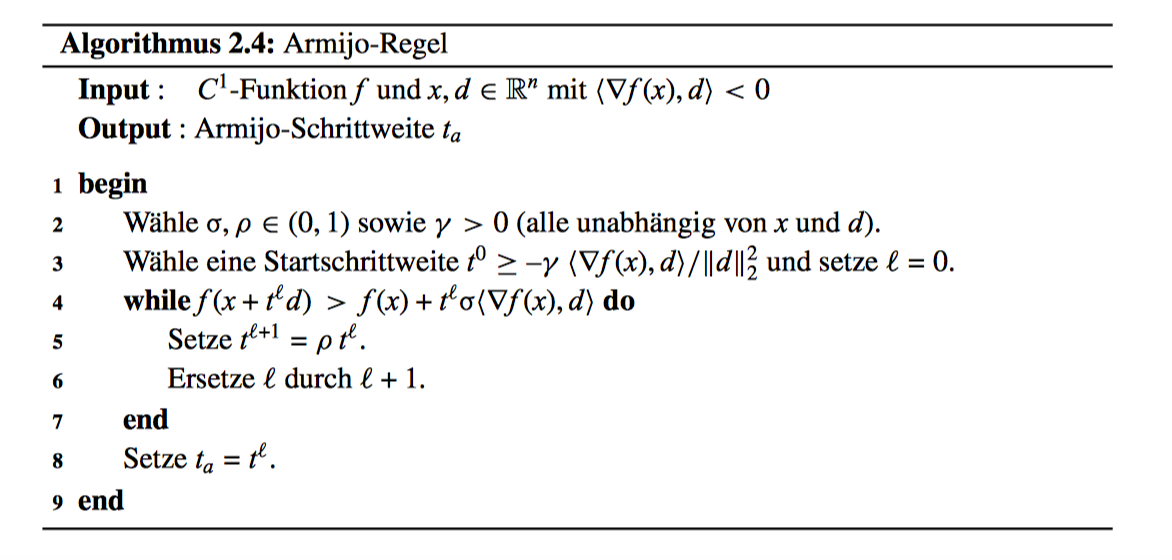
\includegraphics[scale=0.5]{a24}
\end{center}

\begin{satz}
	Die Menge $f_{\leq}^{f(x^0)}$ sei beschränkt, die Funktion $\nabla f$ sei Lipschitz-stetig auf $\operatorname{conv}(f_{\leq}^{f(x^0)})$, und $(d^k)$ sei eine Folge von Abstiegsrichtungen erster Ordnung. Dann ist die Folge der Armijo-Schrittweiten $(t_a^k)$ aus Algorithmus 2.4 (mit unabhängig von $k$ gewählten Parametern $\sigma$, $\rho$ und $\gamma$) wohldefiniert und effizient.
\end{satz}

\begin{uebung}
	Zeigen Sie für die Funktion $f(x) = \frac{1}{2} x^2$, den Startpunkt $x^0 = -3$, die Richtungen $d^k = 2^{-k}$ sowie $\sigma = \frac{1}{2}$, dass der durch die Wahl $t^0 \coloneqq 1$ modifizierte Algorithmus 2.4 nicht zu einer effizienten Schrittweitenfolge führt.
\end{uebung}


Man sollte $t^0$ also so initialisieren, wie in Algorithmus 2.4 angegeben, wobei sich die Wahl $\gamma = 10^{-4}$ bewährt hat. Es ist außerdem nicht schwer zu sehen, dass sich die Armijo-Regel auch für nur einseitig richtungsdifferenzierbare Funktionen einsetzen lässt, indem man das Skalarprodukt $\lambda \nabla f(\overline{x}), d \rangle$ durch $f'(\overline{x}, d)$ ersetzt.

\subsection{Gradientenverfahren}

Aufgrund seiner geometrischen Grundidee ist dies das Verfahren des steilsten Abstiegs.

\begin{center}
	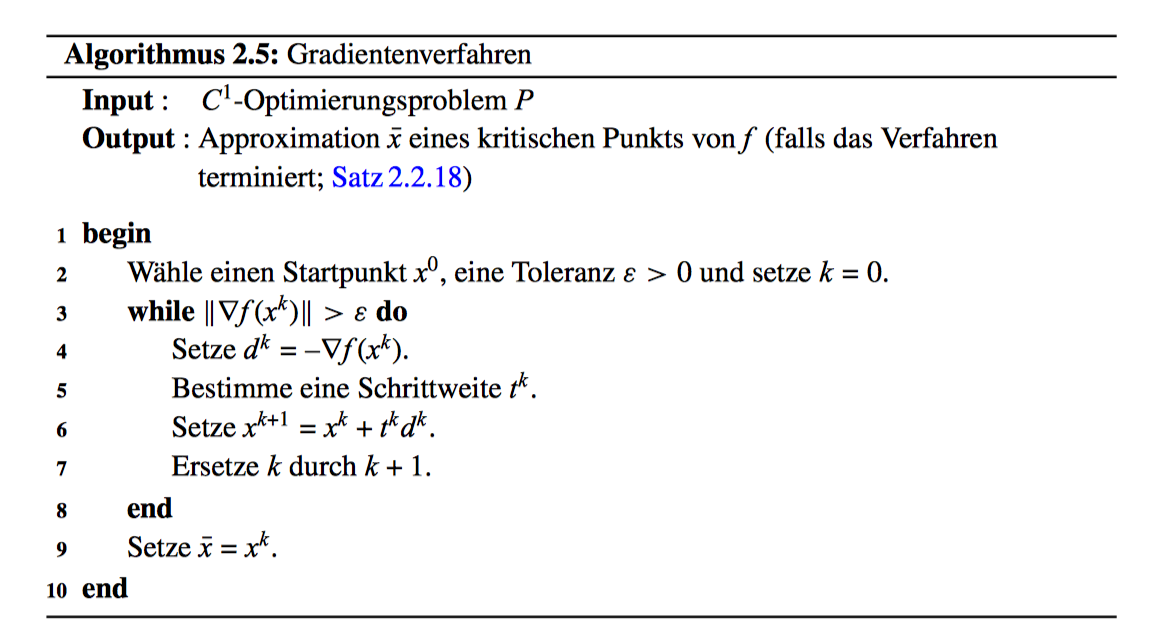
\includegraphics[scale=0.5]{a25}
\end{center}

\begin{satz}
	Die Menge $f_{\leq}^{f(x^0)}$ sei beschränkt, die Funktion $\nabla f$ sei Lipschitz-stetig auf $\operatorname{conv}(f_{\leq}^{f(x^0)})$, und in Zeile 5 seien exakte Schrittweiten $(t_e^k)$ oder Armijo-Schrittweiten $(t_a^k)$ gewählt. Dann terminiert Algorithmus 2.5 für jedes $\epsilon > 0$ nach endlich vielen Schritten. Falls eine Lipschitz-Konstante $L > 0$ zur Lipschitz-Stetigkeit von $\nabla f$ auf $\operatorname{conv}(f_{\leq}^{f(x^0)})$ bekannt ist, dann gilt dieses Ergebnis auch für die dann berechenbaren konstanten Schrittweiten $t_c^k = L^{-1}, k \in \mathbb{N}$.
\end{satz}

\begin{definition*}
	Es ist $\|A\|_2 \coloneqq \max \big\{ \| Ad\|_2 ~|~\| d \|_2 = 1 \big\}$.
\end{definition*}

\begin{uebung}
	Gegeben sei die quadratische Funktion $q(x) = \frac{1}{2} x^T A x + b^T x$ mit $A = A^T$ und $b \in \mathbb{R}^n$. Zeigen Sie, dass der Gradient $\nabla q$ auf ganz $\mathbb{R}^n$ Lipschitz-stetig mit $L = \| A \|_2$ ist. 
\end{uebung}

\begin{beispiel}
	Nach Übung 2.2.19 erzeugt das Gradientenverfahren eine sogar gegen den globalen Minimalpunkt von $q$ konvergente Folge von Iterierten $(x^k)$, wenn entweder exakte, konstante oder Armijo-Schrittweiten gewählt werden. ~\bigskip
	
	Nach Übung 2.2.14 ist bei jeder Abstiegsrichtung erster Ordnung für $q$ in $x$ die (eindeutige) exakte Schrittweite beim Gradientenverfahren 
	$$ t_e = \frac{\| \nabla q(x) \|_2^2}{D q(x) A \nabla q(x)} $$
\end{beispiel}

Falls die Höhenlinien von $f$ die Form lang gezogener Ellipsen mit einem Minimalpunkt $x^*$ in deren gemeinsamem Zentrum besitzen, dann zeigt $-\nabla f(x^k)$ typischerweise nicht in die Richtung von $x^*$. Die Iterierten springen dadurch entlang einer Zickzacklinie, weshalb man in Anlehnung an die englischsprachige Literatur auch vom Zigzagging-Effekt spricht.

\begin{center}
	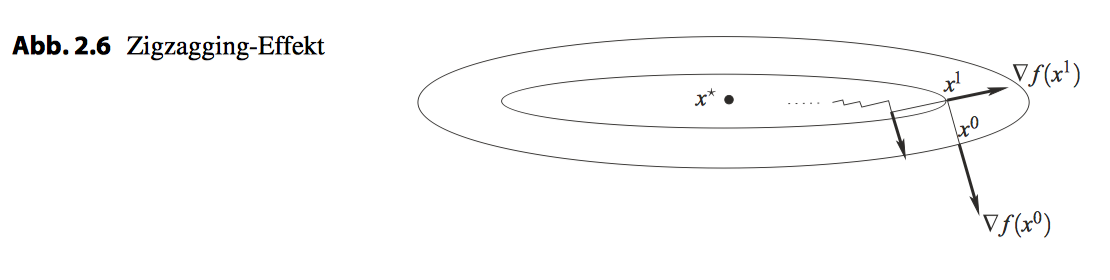
\includegraphics[scale=0.5]{ab26}
\end{center}

\begin{definition}[Konvergenzgeschwindigkeiten]
	Es sei $(x^k)$ eine konvergente Folge mit Grenzpunkt $x^*$. Sie heißt
	\begin{enumerate}[label=\alph*\upshape)]
		\item \textbf{linear konvergent}, falls $\exists 0 < c < 1, ~ k_0 \in \mathbb{N} ~\forall k \geq k_0$: $$ \| x^{k+1} - x^*\| \leq c \cdot \| x^k - x^* \|, $$
		\item \textbf{superlinear konvergent}, falls $\exists c^k \searrow 0, k_0 \in \mathbb{N} ~\forall k \geq k_0$: $$ \| x^{k+1} - x^*\| \leq c^k \cdot \| x^k- x^* \|, $$
		\item \textbf{quadratisch konvergent}, falls $\exists c > 0, k_0 \in \mathbb{N} ~\forall k \geq k_0$: $$ \| x^{k+1} - x^* \| \leq c \cdot \| x^k - x^* \|^2. $$
	\end{enumerate}
\end{definition}

Der folgende Satz zeigt, dass das Gradientenverfahren schon für sehr angenehme Funktionen nur linear konvergente Funktionswerte der Iterierten besitzt, und zwar mit einer Konstante $c$, die sehr nahe bei eins liegen kann. Konkret betrachten wir die konvex-quadratische Funktion $q(x) = \frac{1}{2} x^T A x + b^T x$ mit $A= A^T \succ 0$ sowie $b \in \mathbb{R}^n$ und bezeichnen den größten und den kleinsten Eigenwert der Matrix A mit $\lambda_{max}$ bzw. $\lambda_{min}$ - nach Beispiel 2.2.20 konvergieren dabei die Iterierten des Gradientenverfahrens mit exakten Schrittweiten gegen den globalen Minimalpunkt $x = - A^{-1} b$ von $q$.
    
\begin{lemma}[Kantorowitsch-Ungleichung]
	Es sei $A = A^T \succ 0$ mit maximalem und minimalem Eigenwert $\lambda_{max}$ bzw. $\lambda_{min}$. Dann gilt für jedes $v \in \mathbb{R}^n \setminus \{ 0 \}$
	$$ \frac{v^T A^{-1} v \cdot v^{T} A v}{\| v \|_2^4} \leq \frac{\left(\lambda_{max}+ \lambda_{min} \right)^2}{4 \lambda_{max} \lambda_{min}} $$
\end{lemma}

\begin{satz}
	Auf die konvex-quadratische Funktion $q(x) = \frac{1}{2} x^T A x + b^T x$ mit $A = A^T \succ 0$ und $b \in \mathbb{R}^n$ werde das Gradientenverfahren mit exakten Schrittweiten und $\epsilon = 0$ angewendet. Dann gilt für alle $k \in \mathbb{N}$
	$$ |q(x^{k+1}) - q(x^*)| \leq \left( \frac{\lambda_{max} - \lambda_{min}}{\lambda_{max} + \lambda_{min}} \right)^2 |q(x^k) - q(x^*)|. $$
\end{satz}

\end{document}